\documentclass[letterpaper]{article}
\usepackage{lmodern}
\usepackage{amssymb,amsmath}
\usepackage{ifxetex,ifluatex}
\usepackage{fixltx2e} % provides \textsubscript
\ifnum 0\ifxetex 1\fi\ifluatex 1\fi=0 % if pdftex
  \usepackage[T1]{fontenc}
  \usepackage[utf8]{inputenc}
\else % if luatex or xelatex
  \ifxetex
    \usepackage{mathspec}
    \usepackage{xltxtra,xunicode}
  \else
    \usepackage{fontspec}
  \fi
  \defaultfontfeatures{Mapping=tex-text,Scale=MatchLowercase}
  \newcommand{\euro}{€}
\fi
% use upquote if available, for straight quotes in verbatim environments
\IfFileExists{upquote.sty}{\usepackage{upquote}}{}
% use microtype if available
\IfFileExists{microtype.sty}{%
\usepackage{microtype}
\UseMicrotypeSet[protrusion]{basicmath} % disable protrusion for tt fonts
}{}
\usepackage[margin=1.5cm]{geometry}
\usepackage{graphicx}
\makeatletter
\def\maxwidth{\ifdim\Gin@nat@width>\linewidth\linewidth\else\Gin@nat@width\fi}
\def\maxheight{\ifdim\Gin@nat@height>\textheight\textheight\else\Gin@nat@height\fi}
\makeatother
% Scale images if necessary, so that they will not overflow the page
% margins by default, and it is still possible to overwrite the defaults
% using explicit options in \includegraphics[width, height, ...]{}
\setkeys{Gin}{width=\maxwidth,height=\maxheight,keepaspectratio}
\ifxetex
  \usepackage[setpagesize=false, % page size defined by xetex
              unicode=false, % unicode breaks when used with xetex
              xetex]{hyperref}
\else
  \usepackage[unicode=true]{hyperref}
\fi
\hypersetup{breaklinks=true,
            bookmarks=true,
            pdfauthor={},
            pdftitle={},
            colorlinks=true,
            citecolor=blue,
            urlcolor=blue,
            linkcolor=magenta,
            pdfborder={0 0 0}}
\urlstyle{same}  % don't use monospace font for urls
\setlength{\parindent}{0pt}
\setlength{\parskip}{6pt plus 2pt minus 1pt}
\setlength{\emergencystretch}{3em}  % prevent overfull lines
\setcounter{secnumdepth}{0}

%%% Use protect on footnotes to avoid problems with footnotes in titles
\let\rmarkdownfootnote\footnote%
\def\footnote{\protect\rmarkdownfootnote}

%%% Change title format to be more compact
\usepackage{titling}

% Create subtitle command for use in maketitle
\newcommand{\subtitle}[1]{
  \posttitle{
    \begin{center}\large#1\end{center}
    }
}

\setlength{\droptitle}{-2em}
  \title{}
  \pretitle{\vspace{\droptitle}}
  \posttitle{}
  \author{}
  \preauthor{}\postauthor{}
  \date{}
  \predate{}\postdate{}



\begin{document}

\maketitle


\setlength{\unitlength}{1in} \fontfamily{phv}\selectfont

\graphicspath{{../../../results/master_output/heatmaps/}}
\textbf{\LARGE{Figure 1}}

\begin{picture}(0,4.5)
\put(0.1,-0.5){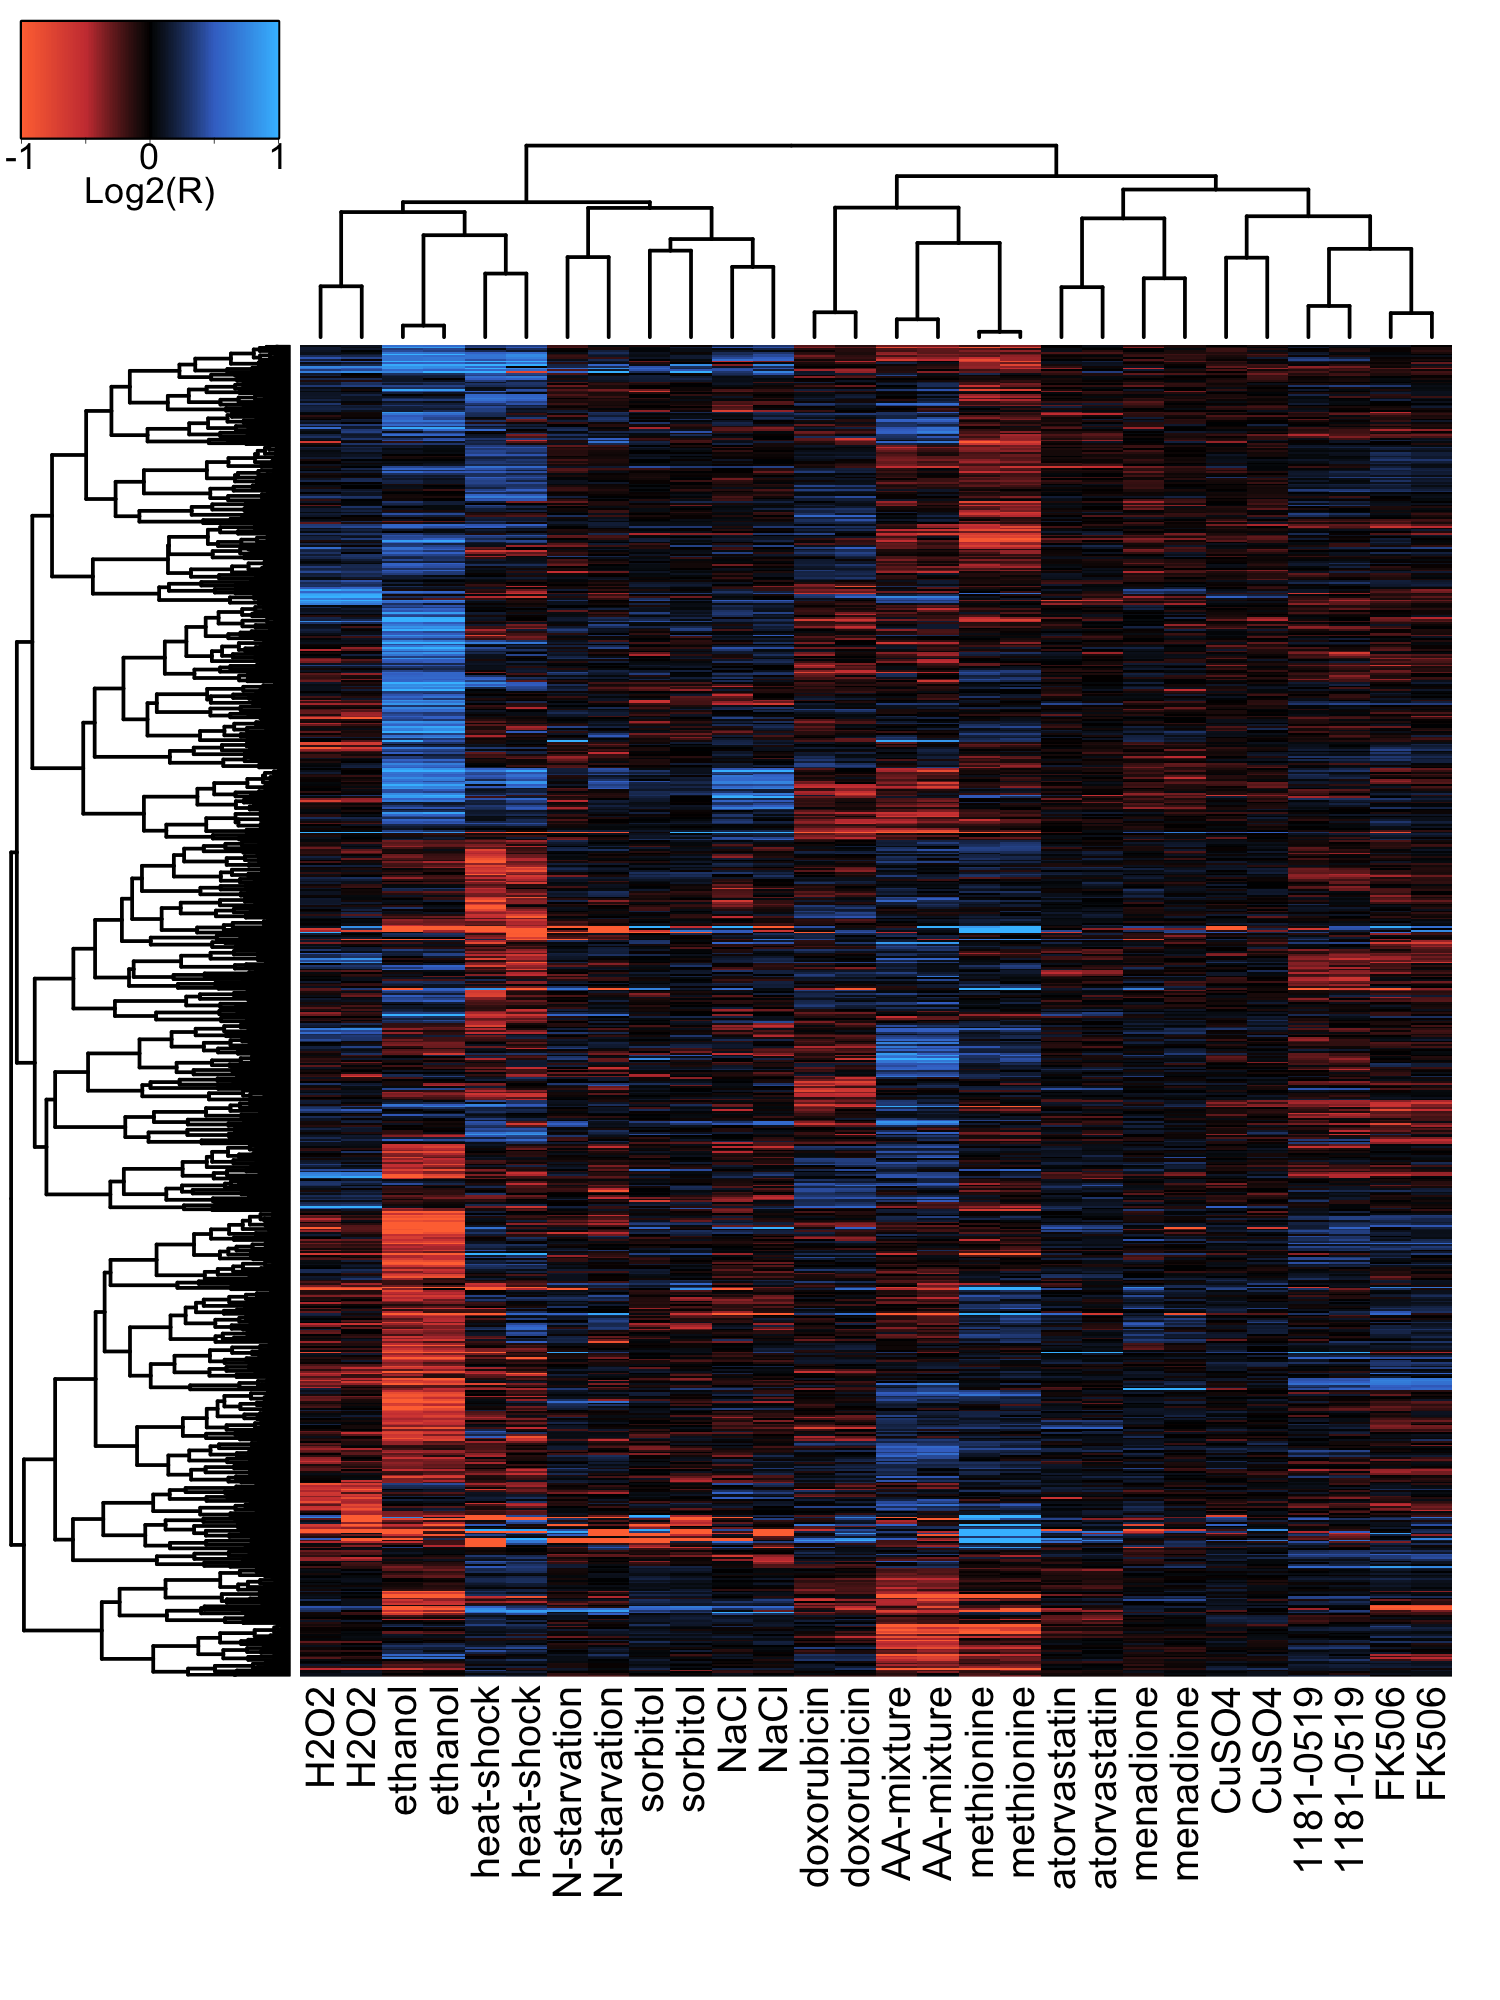
\includegraphics[width=3.5in]{all_sig_bpcs.png}}
\put(3.7,0.45){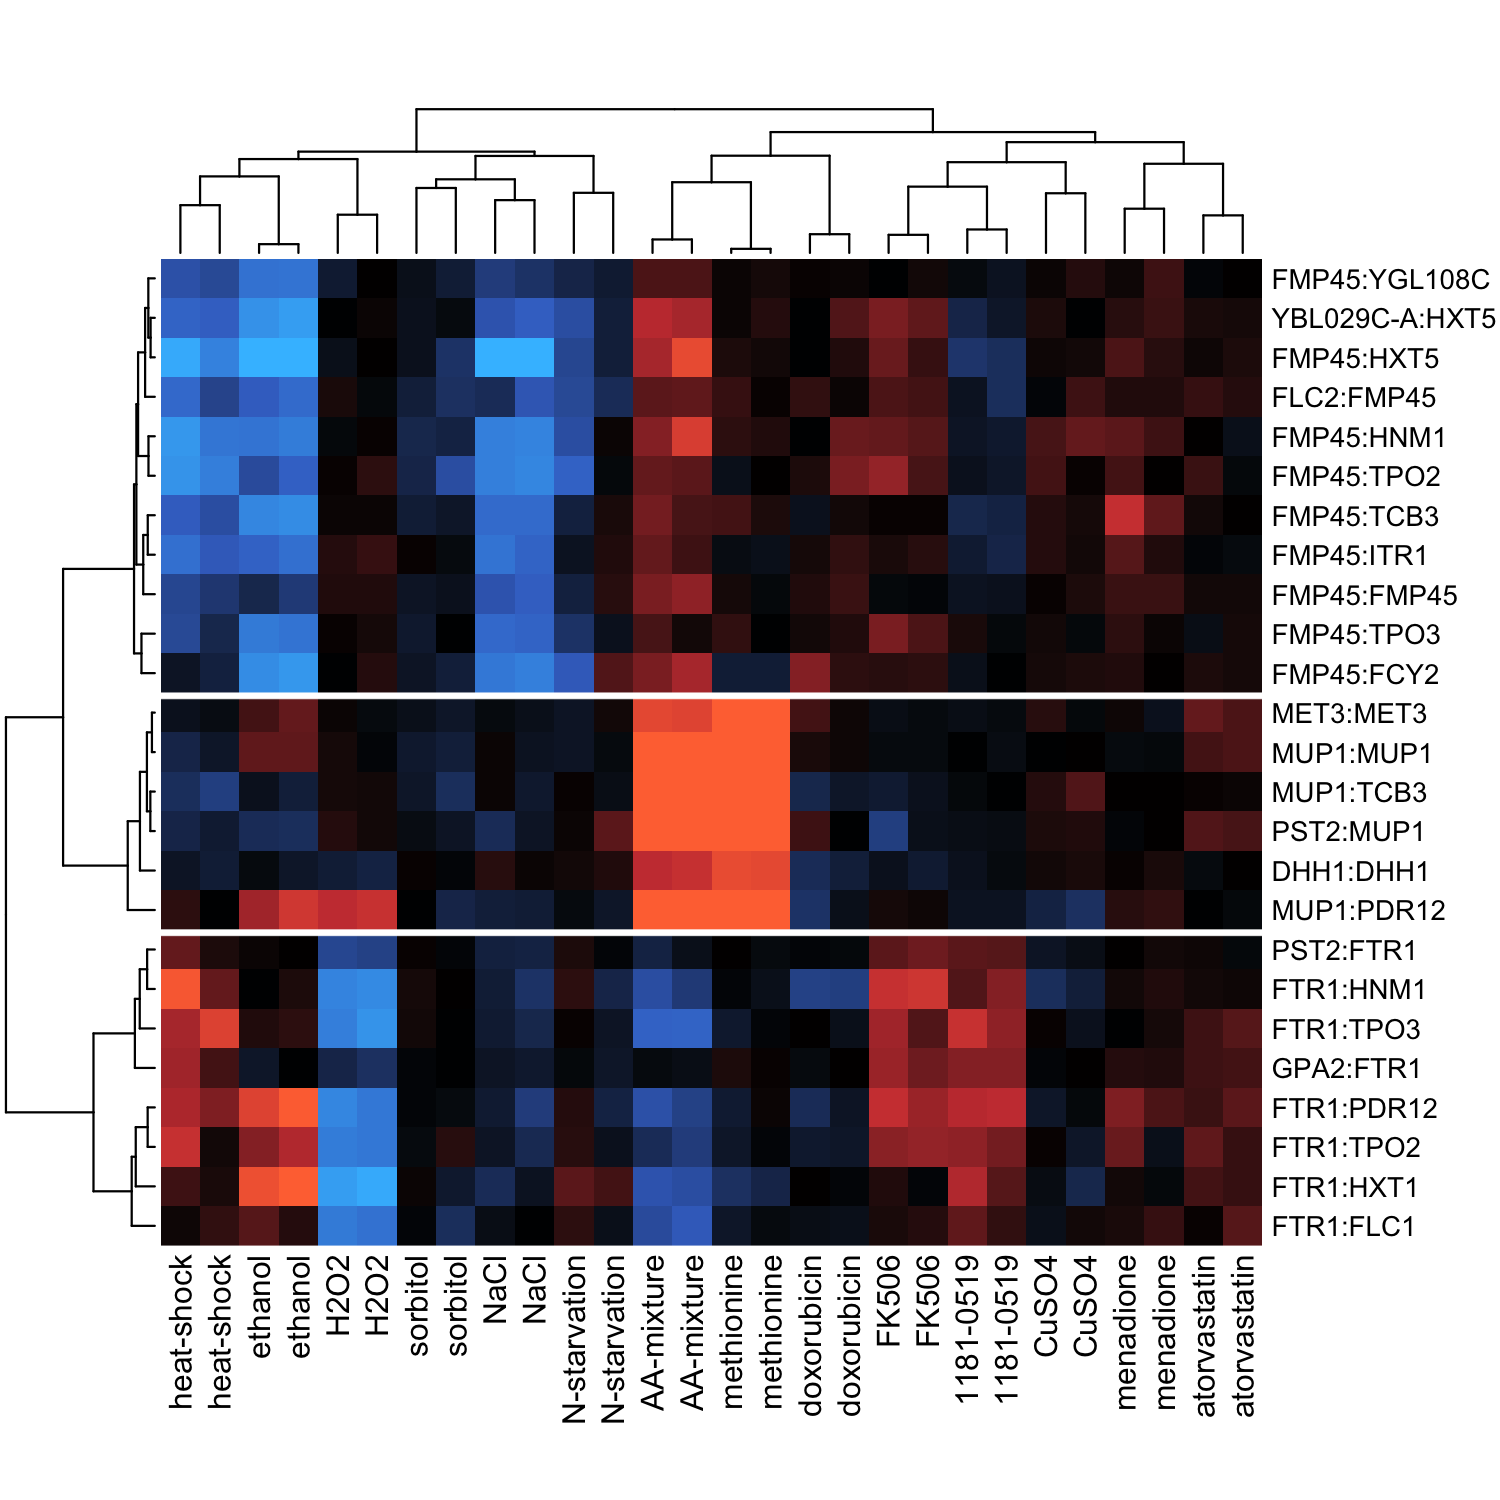
\includegraphics[width=3.5in]{clusters_sig_bpcs.png}}
\put(0.1,-3){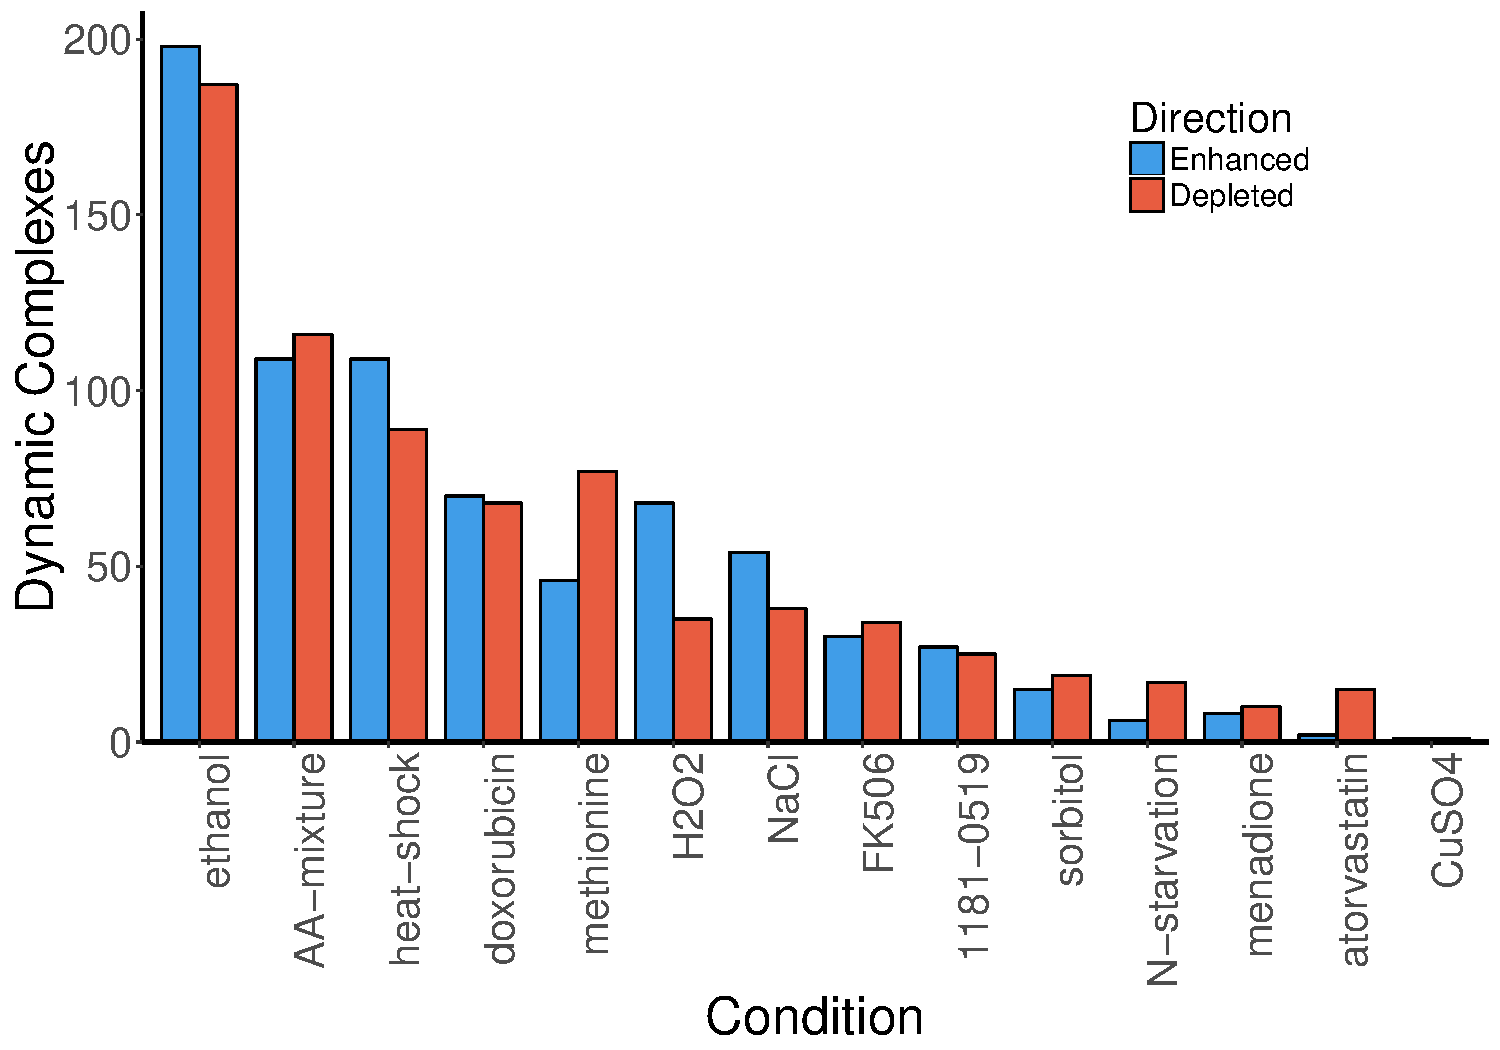
\includegraphics[width=3.5in]{number_dynamic_bpcs.pdf}}
\put(0,4.2){\textbf{A}}
\put(3.7,4.2){\textbf{B}}
\put(0,-0.5){\textbf{C}}
\end{picture}

\newpage

\graphicspath{{../../../results/external_graphics/go_enrichment/}}
\textbf{\LARGE{Figure 2}}

\begin{picture}(0,4.5)
\put(0,1.65){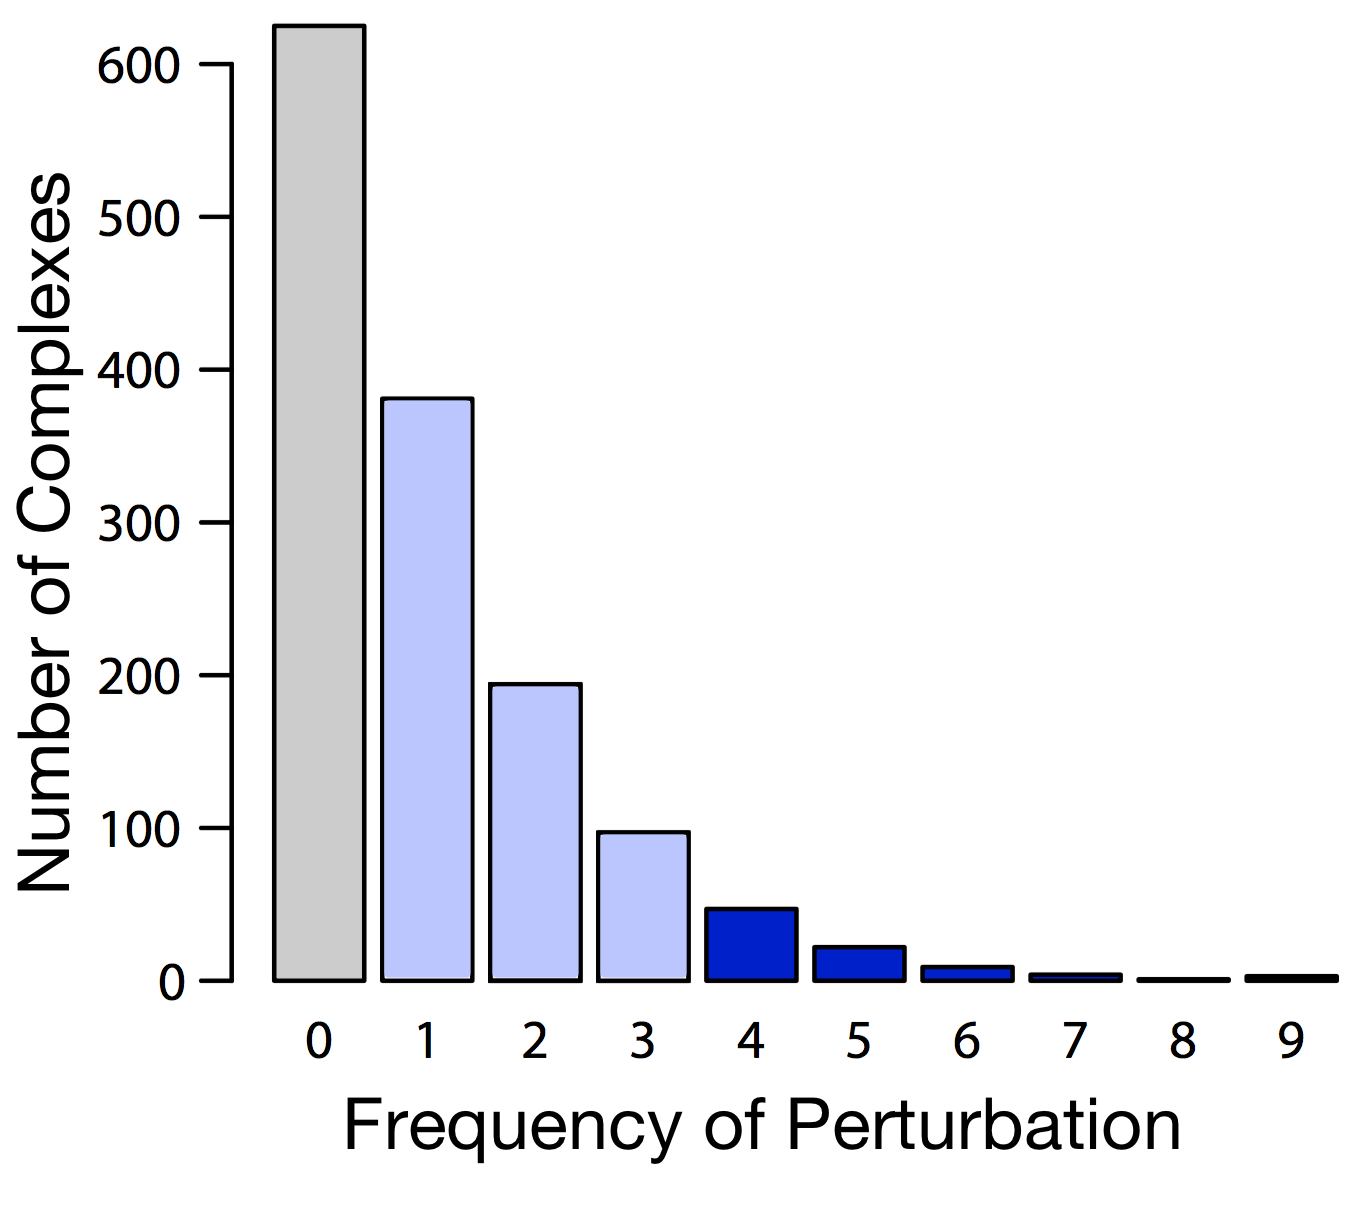
\includegraphics[width=3in]{fig_2a.png}}
\put(3.5,1.65){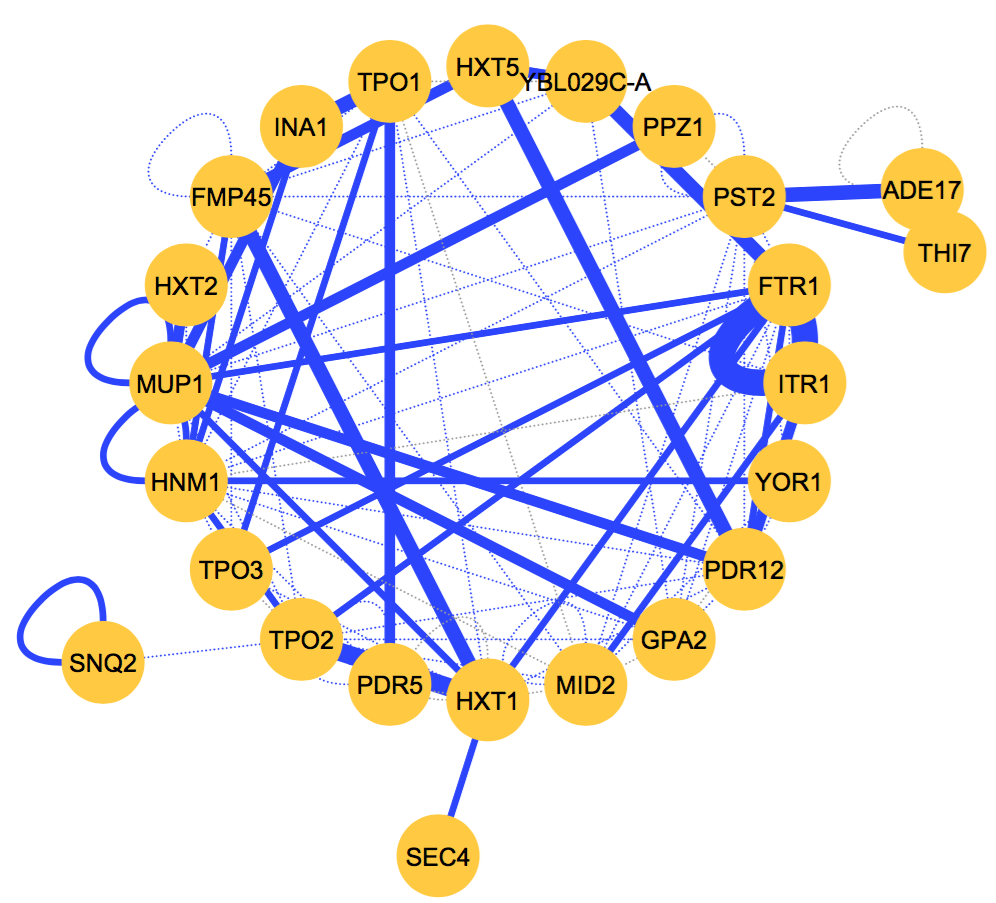
\includegraphics[width=3in]{fig_2b.png}}

\put(0.1,-2.2){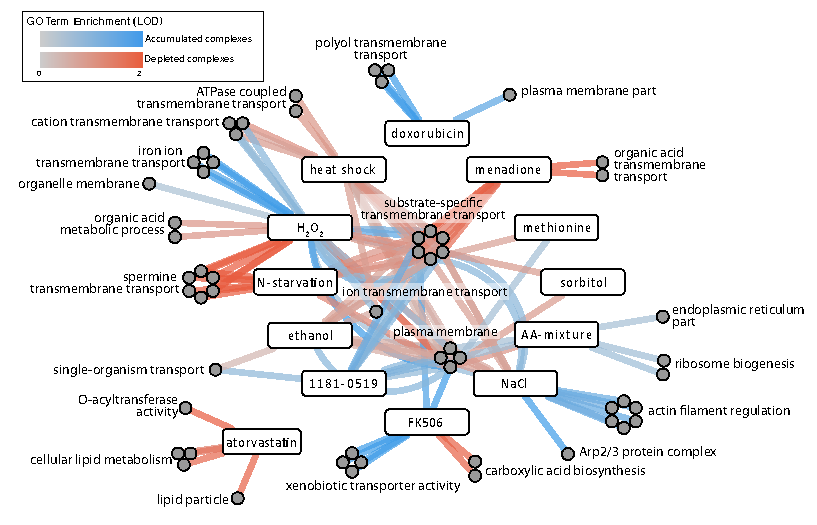
\includegraphics[width=10in]{node_enrichment_go_v2_1.pdf}}
\put(0,4.2){\textbf{A}}
\put(3.5,4.2){\textbf{B}}
\put(0,1.2){\textbf{C}}
\end{picture}

\newpage
 \textbf{\LARGE{Figure 3}}
\graphicspath{{../../../results/master_output/connectivity/}}

\begin{picture}(0,4.5)
\put(3.6,-0.75){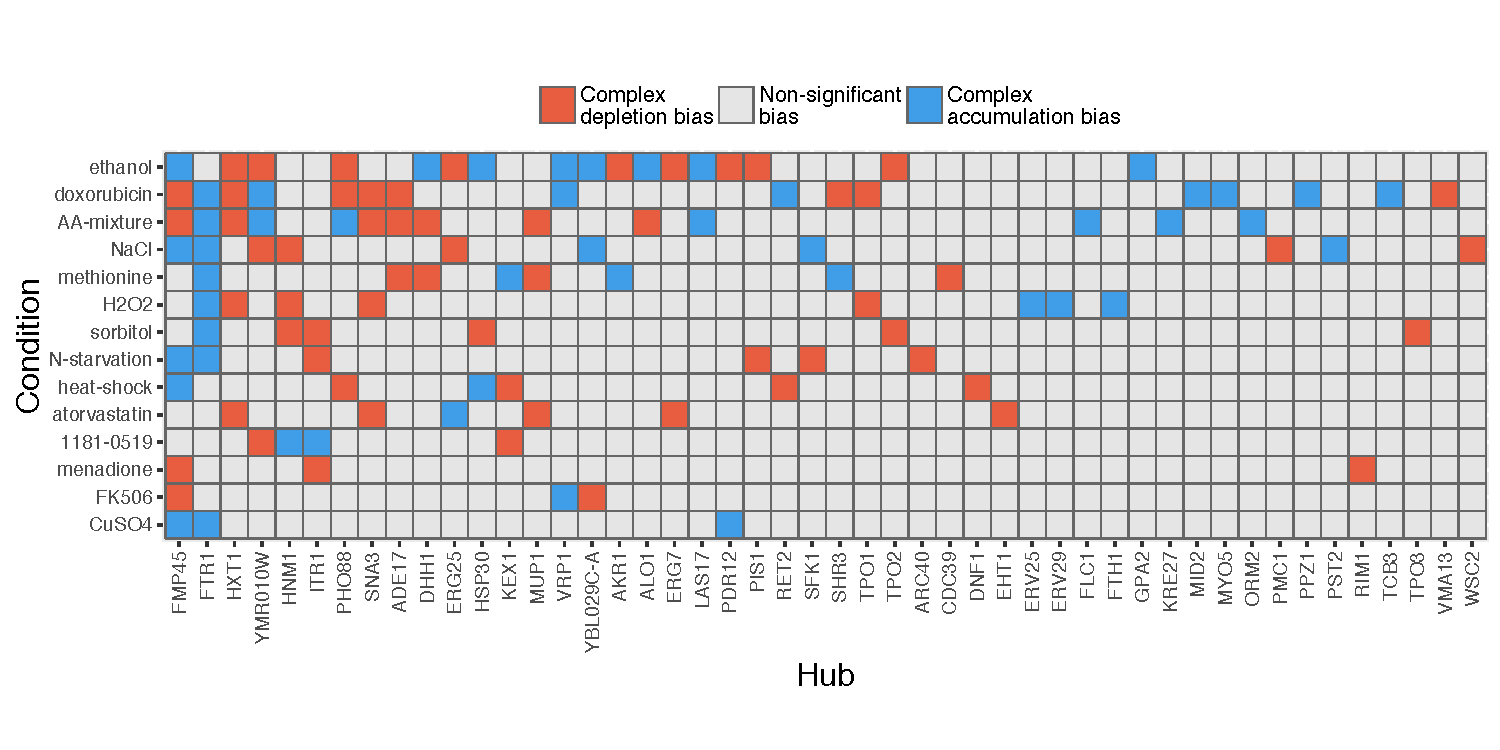
\includegraphics[width=3.5in]{hub_bias_heatmap.pdf}}
\put(0,-0.5){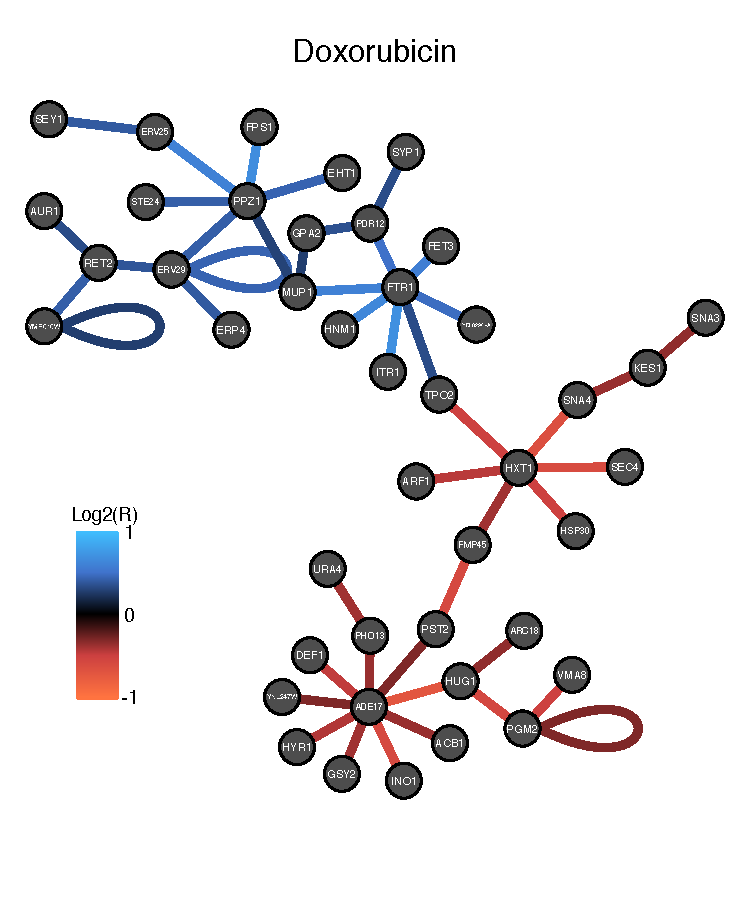
\includegraphics[width=4in]{doxorubicin_connnectivity.pdf}}
\put(0,-3.91){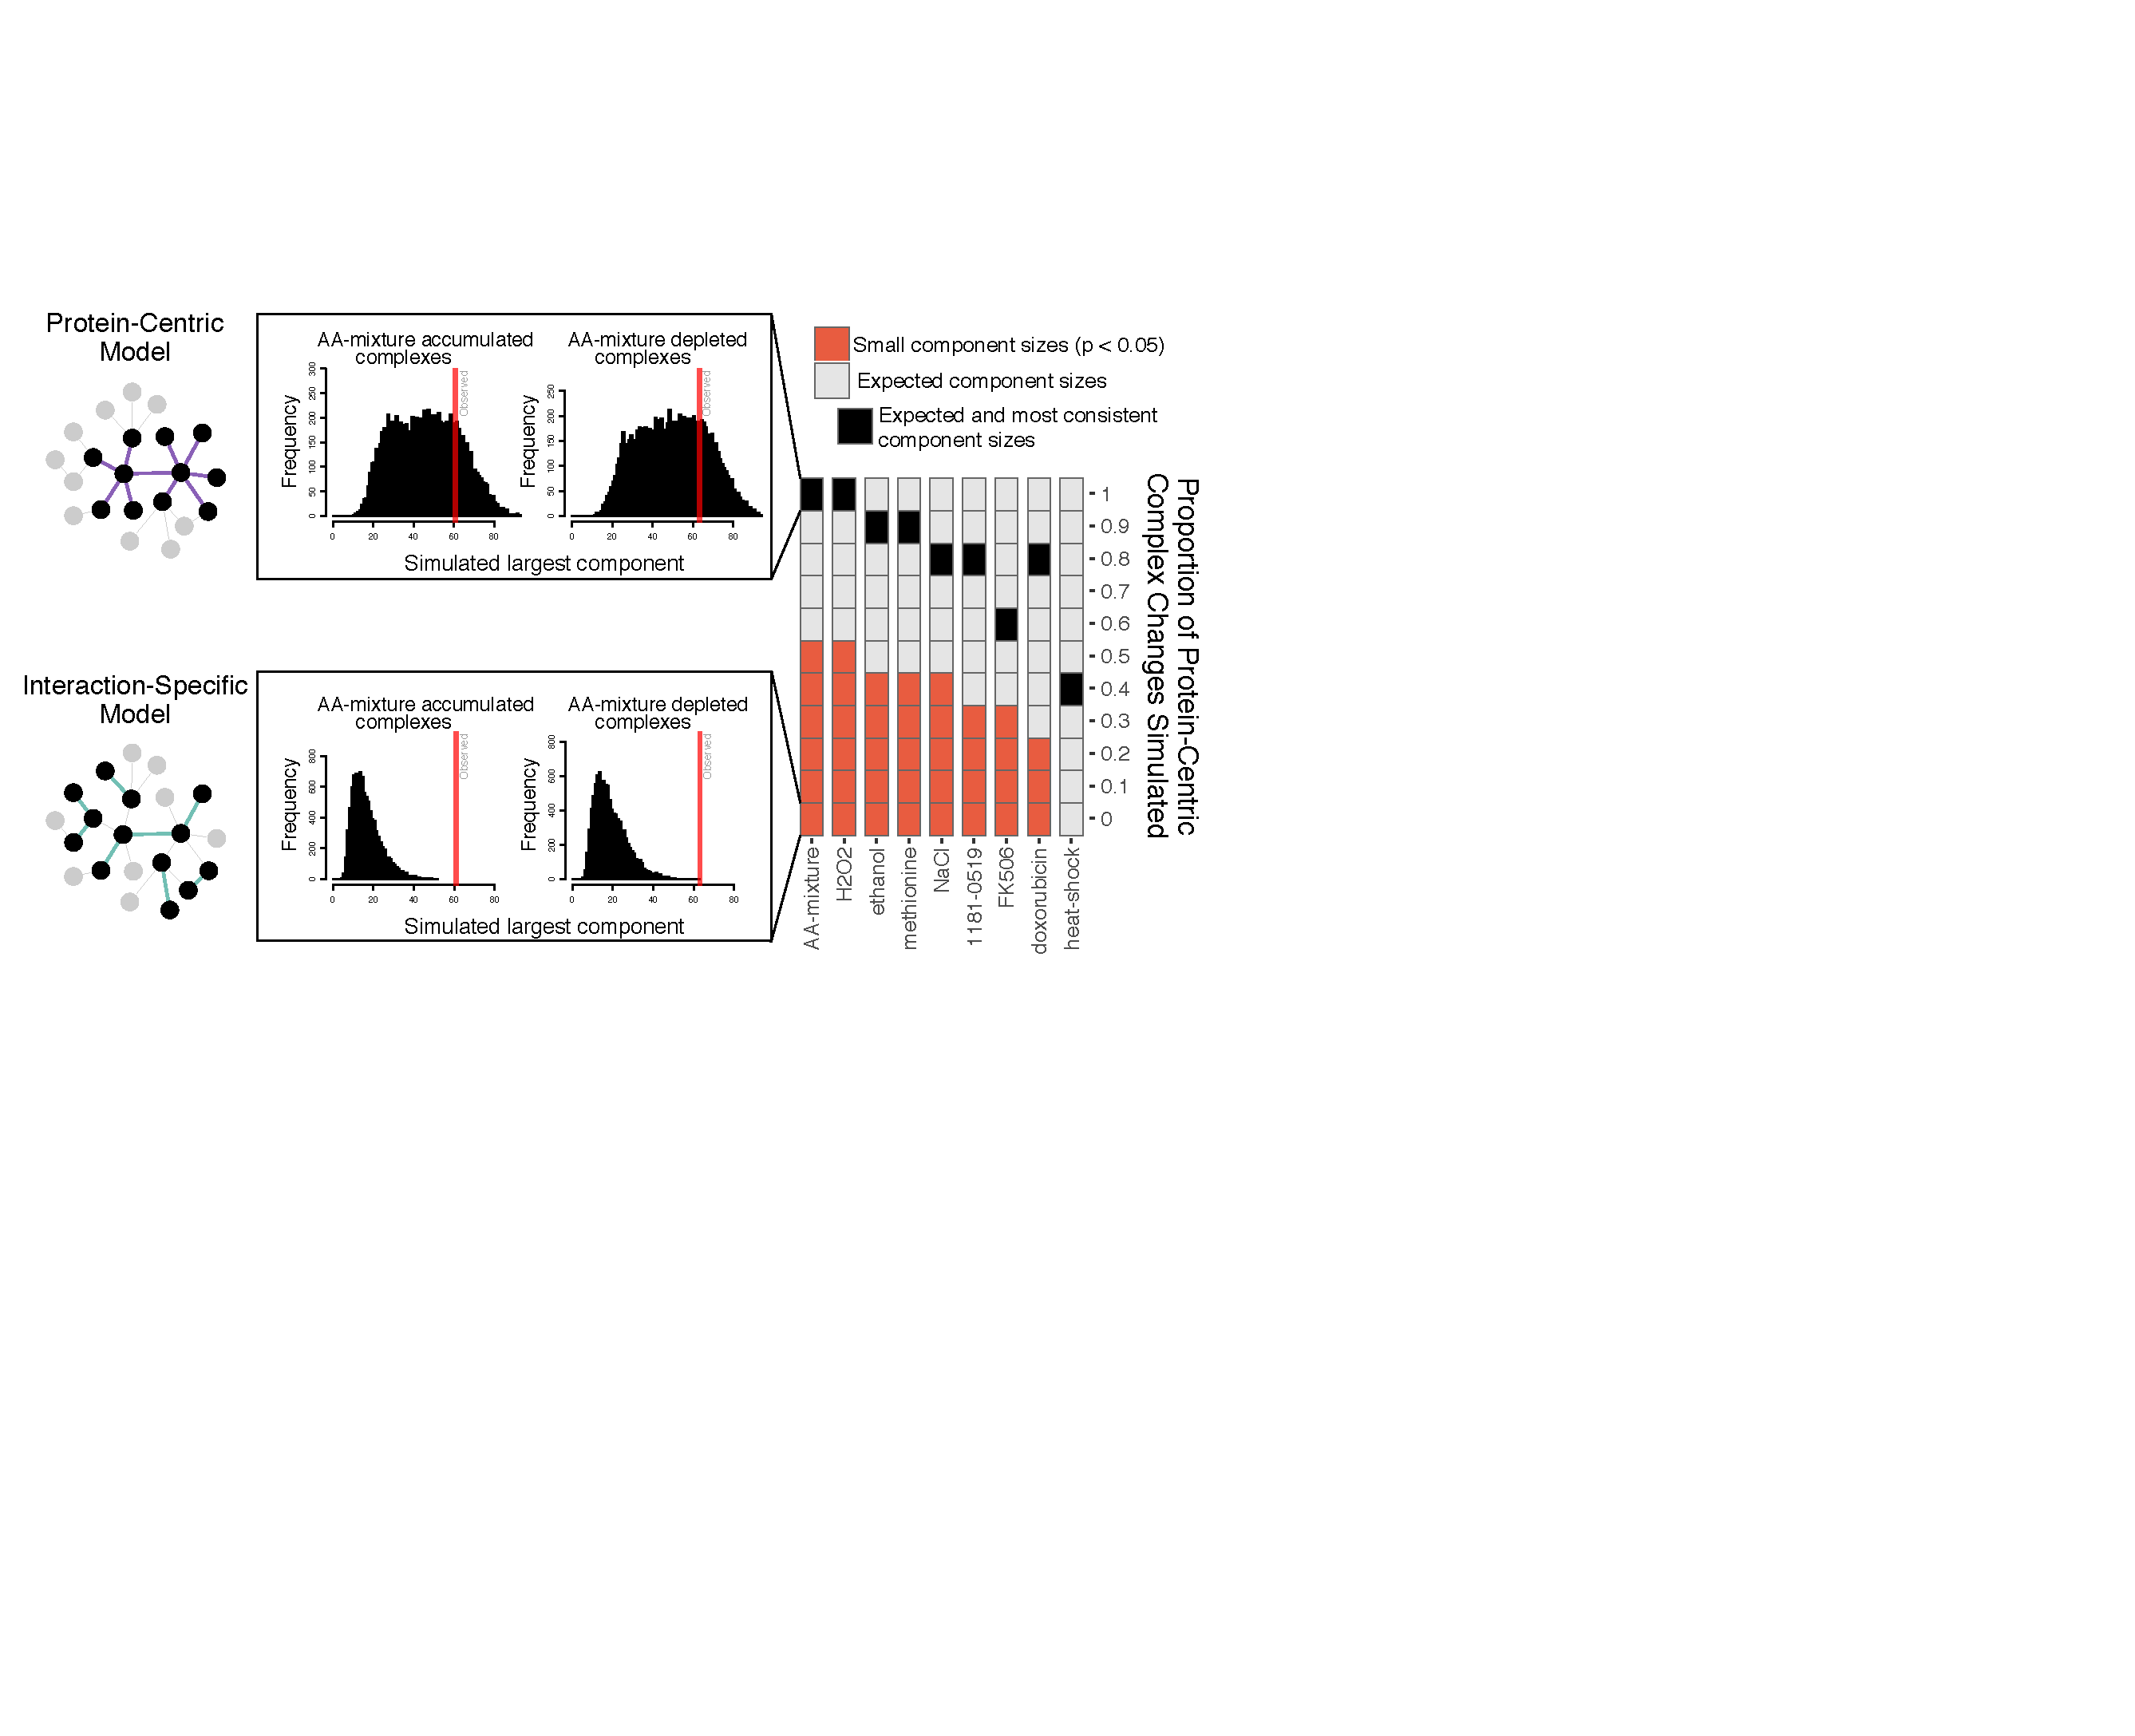
\includegraphics[width=4.9in]{component_size_significance_search.pdf}}
\put(3.9,-3.7){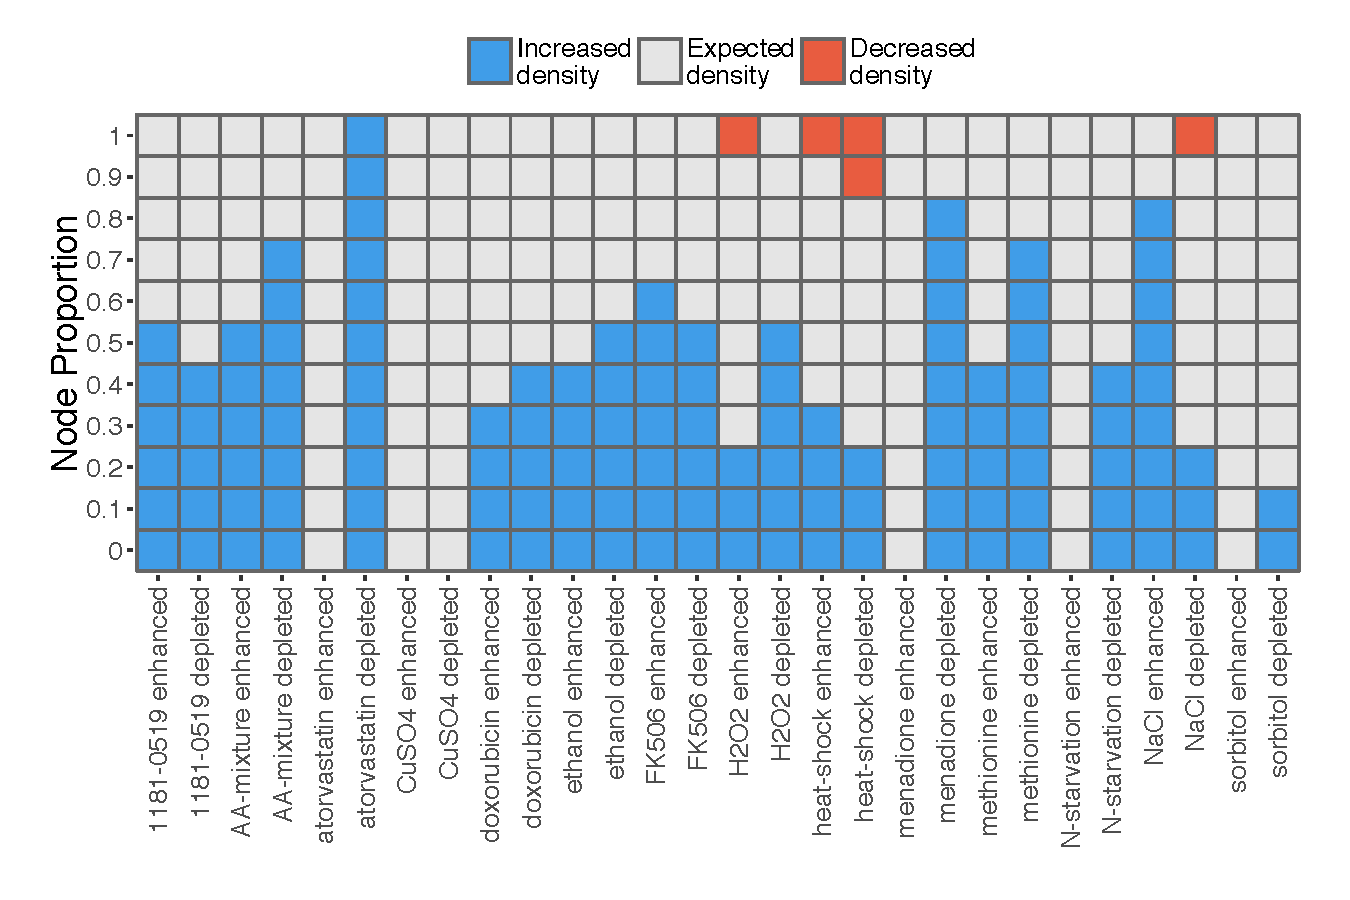
\includegraphics[width=4.3in]{density_significance_search.pdf}}
\graphicspath{{../../../results/external_graphics/node_edge_simulation/}}
\put(2.7,-3.3){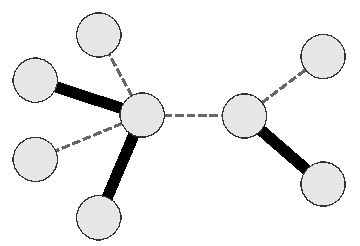
\includegraphics[width=0.7in]{all_edge.pdf}}
\put(2.7,-1.7){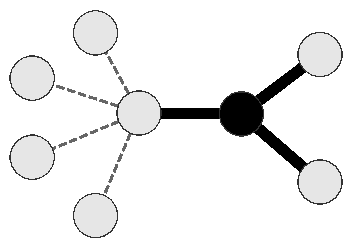
\includegraphics[width=0.7in]{all_node.pdf}}
\put(6.45,-3.3){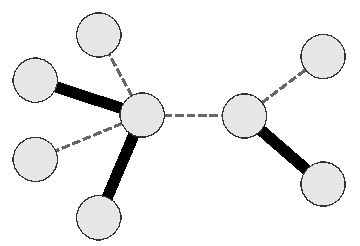
\includegraphics[width=0.7in]{all_edge.pdf}}
\put(6.45,-1.7){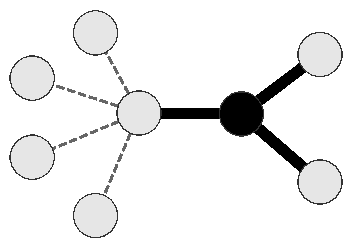
\includegraphics[width=0.7in]{all_node.pdf}}
\put(0,4.1){\textbf{A}}
\put(4,4.1){\textbf{B}}
\put(0,-1.3){\textbf{C}}
\put(4,-1.3){\textbf{D}}
\end{picture}

\newpage

\graphicspath{{../../../results/master_output/expression_pca/}}
\textbf{\LARGE{Figure 4}}

\begin{picture}(0,4.5)
\put(0,1.25){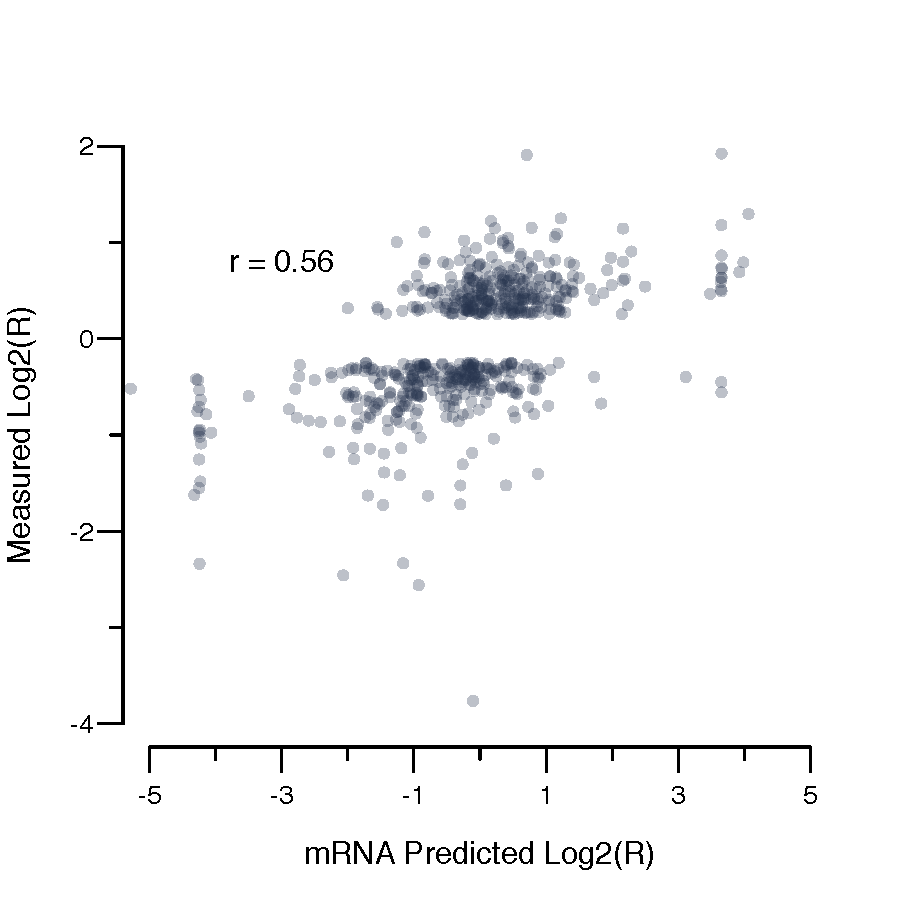
\includegraphics[width=3.3in]{bcPCA_predictions_significant_filtered.pdf}}
\put(4,1.25){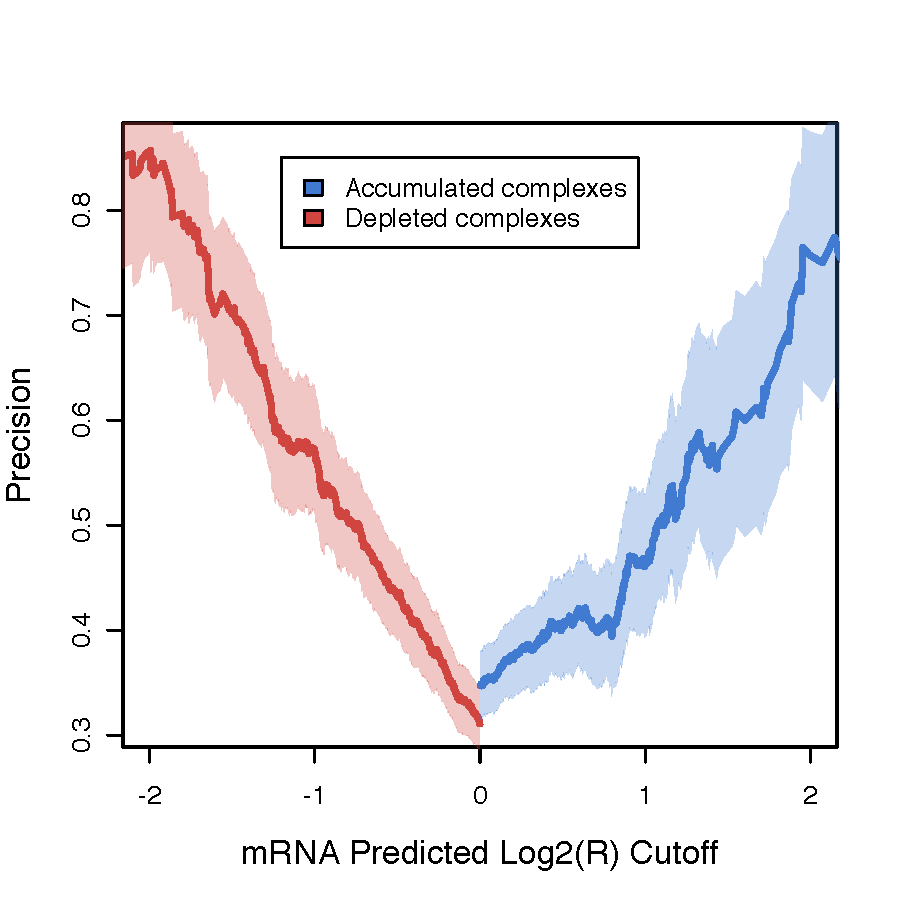
\includegraphics[width=3.3in]{bcPCA_precision.pdf}}

\put(0,-4){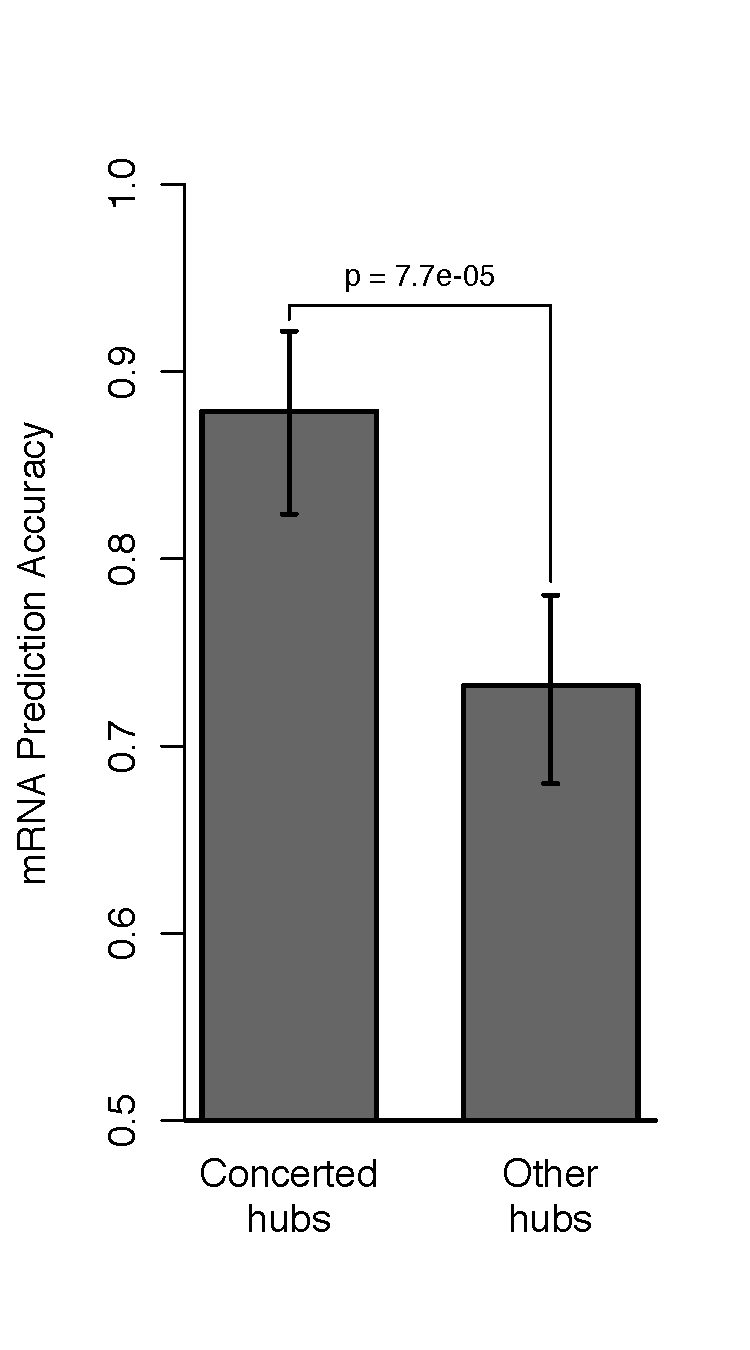
\includegraphics[width=2in]{hub_comparison.pdf}}
\put(0,-0.5){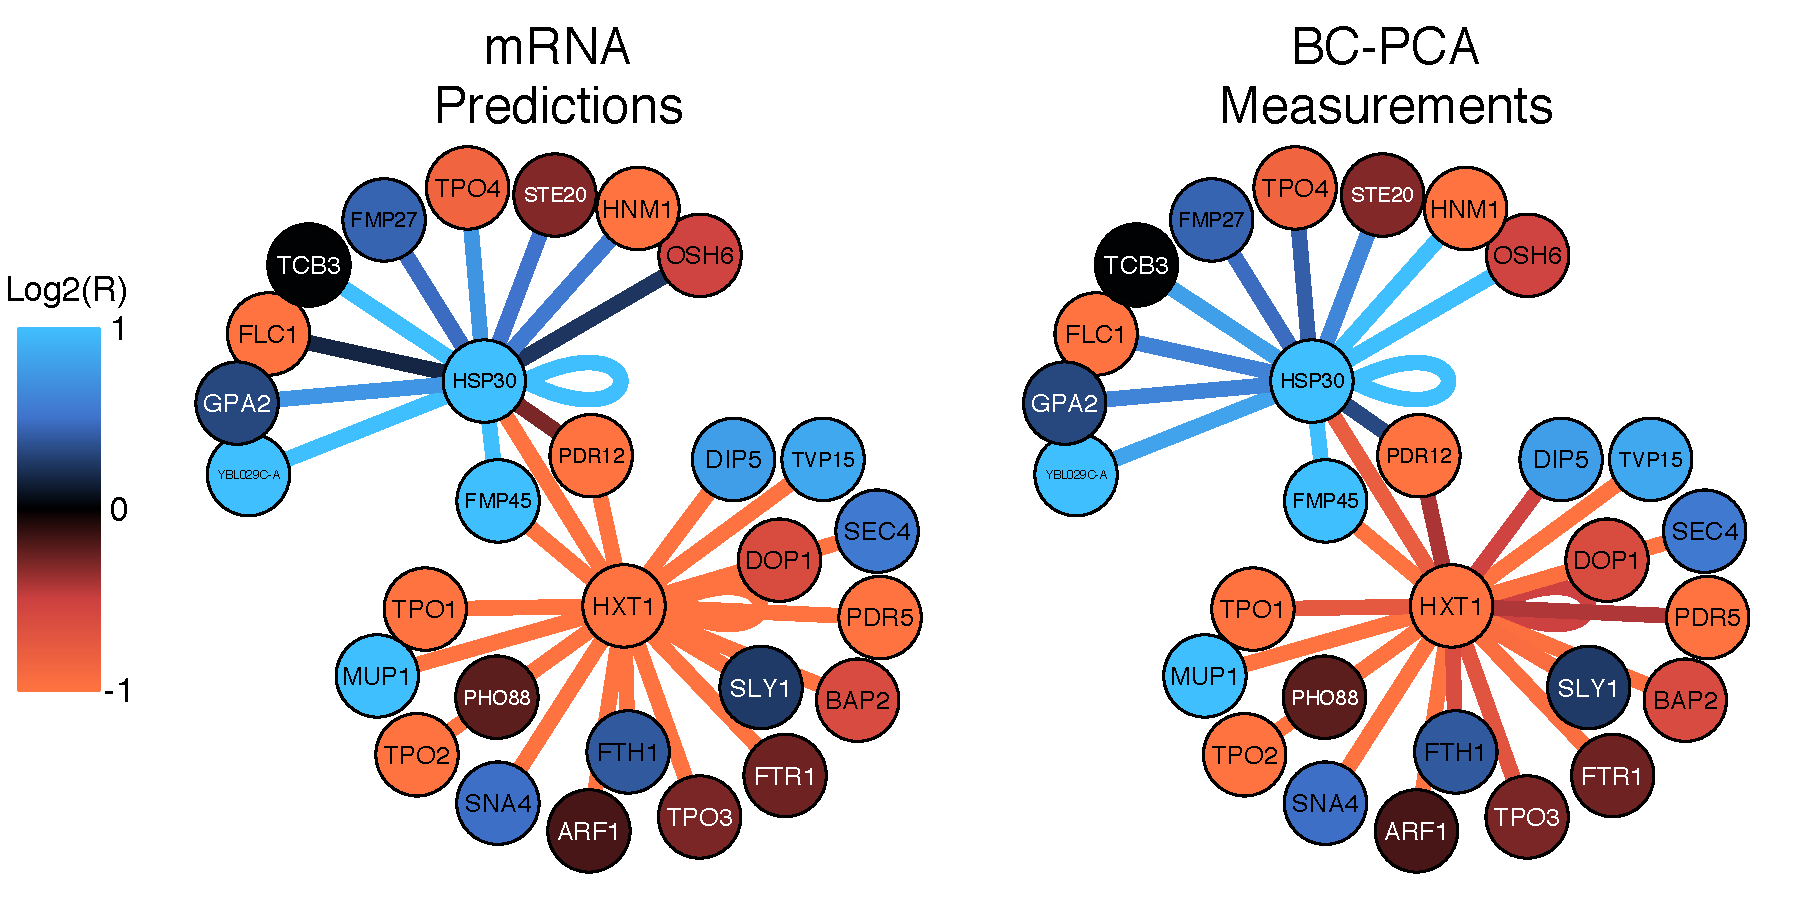
\includegraphics[width=3.5in]{HXT1_HSP30_comparison.pdf}}
\put(3.8,-0.5){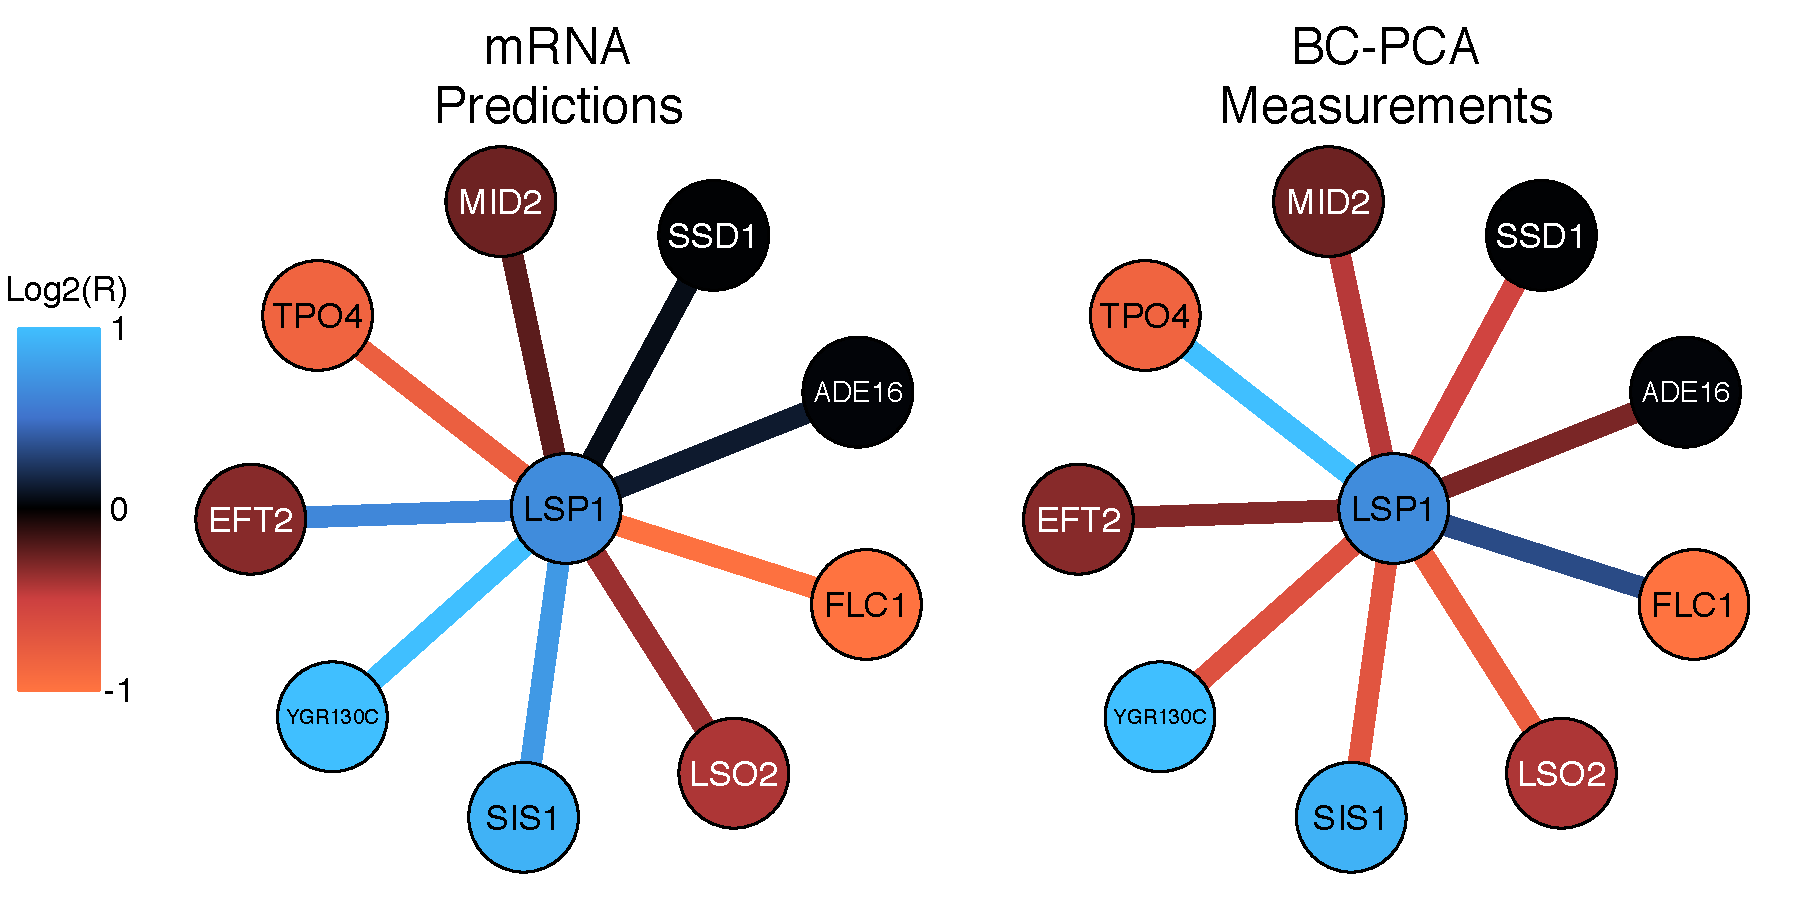
\includegraphics[width=3.5in]{LSP1_comparison.pdf}}

\graphicspath{{../../../results/external_graphics/}}
\put(2.4,-4.1){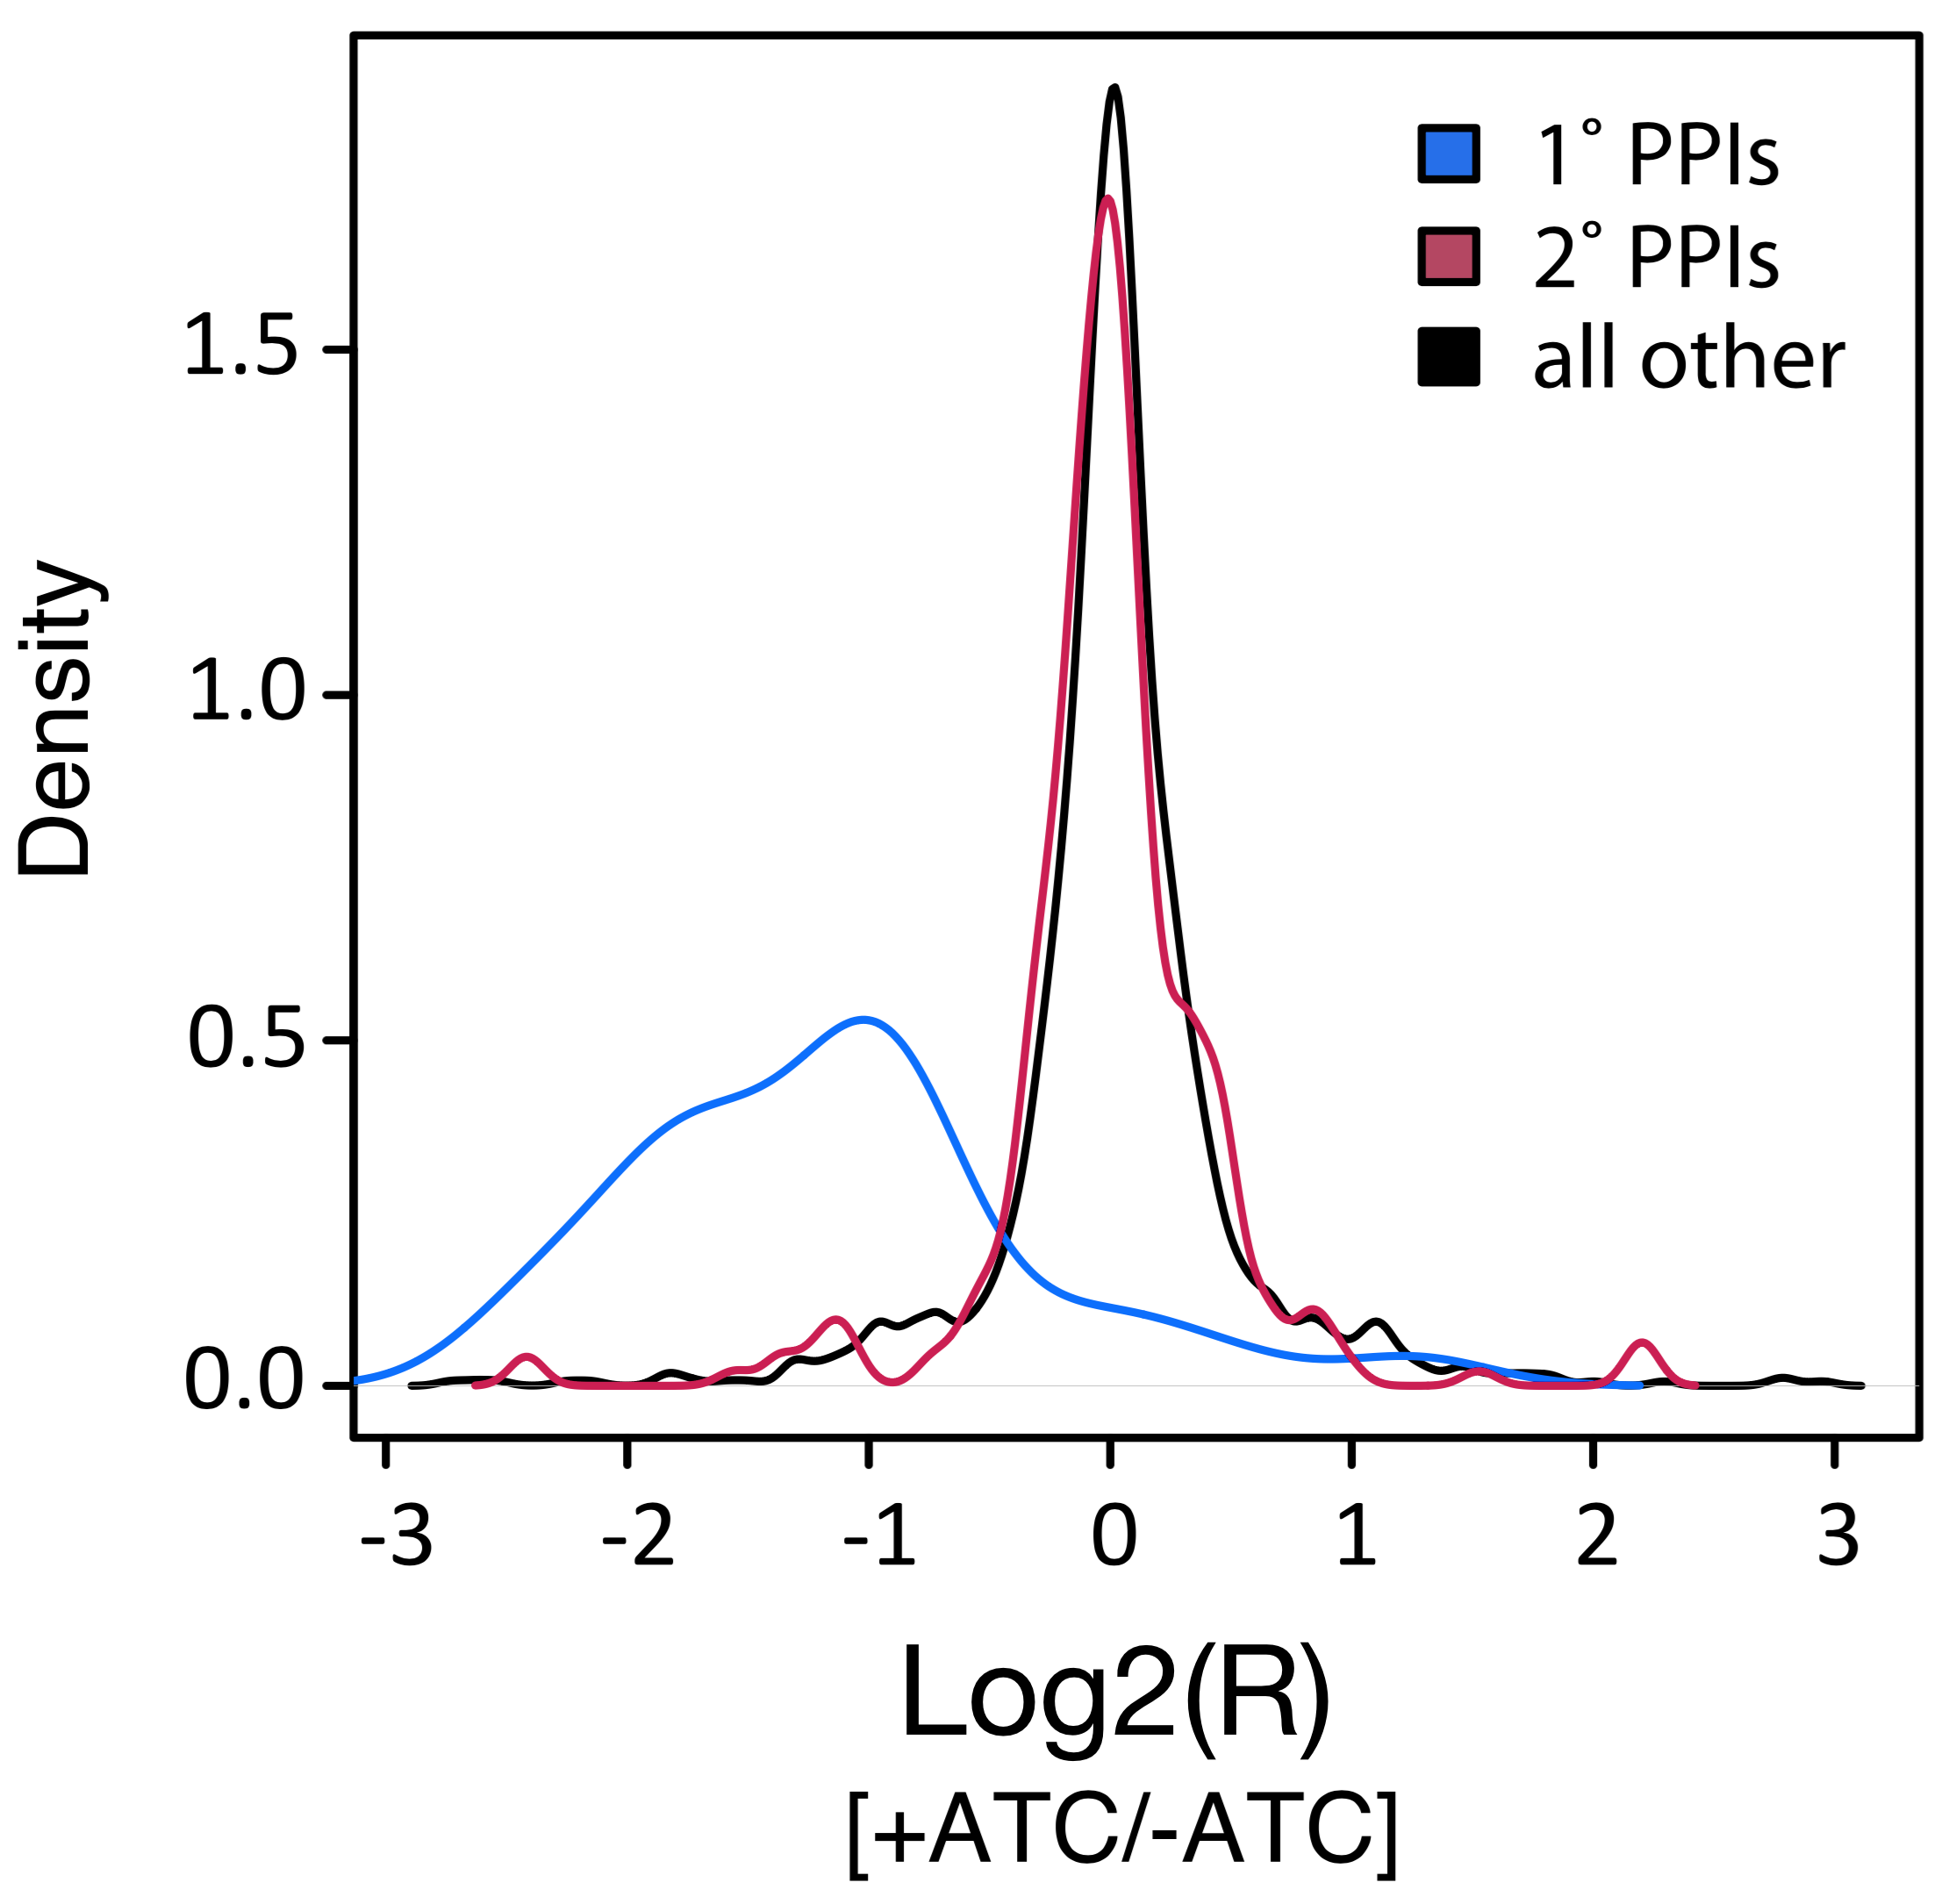
\includegraphics[width=3.2in]{primary_vs_secondary.png}}
\put(0,4){\textbf{A}}
\put(3.8,4){\textbf{B}}
\put(0,1.1){\textbf{C}}
\put(3.8,1.1){\textbf{D}}
\put(0,-0.8){\textbf{E}}
\put(2.5,-0.8){\textbf{F}}

\end{picture}

\end{document}
